% Auto-generated by paper/latex/scripts/generate_latex_data.js
\begin{figure}[t]
\centering
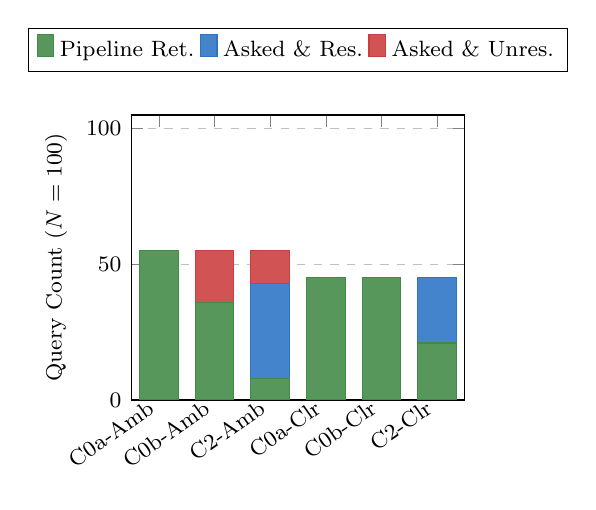
\begin{tikzpicture}[font=\footnotesize]
  % Define colors
  \definecolor{cPipeline}{RGB}{46, 125, 50}
  \definecolor{cResolved}{RGB}{21, 101, 192}
  \definecolor{cUnresolved}{RGB}{198, 40, 40}

  \begin{axis}[
    ybar stacked,
    bar width=14pt,
    width=0.48\textwidth,
    height=5.2cm,
    ymin=0, ymax=105,
    ylabel={Query Count ($N = 100$)},
    symbolic x coords={C0a-Amb, C0b-Amb, C2-Amb, C0a-Clr, C0b-Clr, C2-Clr},
    xtick=data,
    x tick label style={rotate=35, anchor=east},
    legend style={at={(0.5,1.15)}, anchor=south, legend columns=3},
    ymajorgrids=true,
    grid style=dashed,
  ]
  % 1. Pipeline Returned (Direct Execution)
  \addplot[fill=cPipeline!80, draw=cPipeline!90] coordinates {
    (C0a-Amb, 55) (C0b-Amb, 36) (C2-Amb, 8)
    (C0a-Clr, 45) (C0b-Clr, 45) (C2-Clr, 21)
  };
  \addlegendentry{Pipeline Ret.}

  % 2. Asked & Resolved (Interactive Disambiguation)
  \addplot[fill=cResolved!80, draw=cResolved!90] coordinates {
    (C0a-Amb, 0) (C0b-Amb, 0) (C2-Amb, 35)
    (C0a-Clr, 0) (C0b-Clr, 0) (C2-Clr, 24)
  };
  \addlegendentry{Asked \& Res.}

  % 3. Asked & Unresolved (Model / User Abort)
  \addplot[fill=cUnresolved!80, draw=cUnresolved!90] coordinates {
    (C0a-Amb, 0) (C0b-Amb, 19) (C2-Amb, 12)
    (C0a-Clr, 0) (C0b-Clr, 0) (C2-Clr, 0)
  };
  \addlegendentry{Asked \& Unres.}
  \end{axis}
\end{tikzpicture}
\caption{Distribution of generation outcomes across ambiguous ($n = 55$) and clear ($n = 45$) queries under C0a (Zero-ARL), C0b (LLM-Only), and C2 (AtlasMind Gate).}
\label{fig:outcomes}
\end{figure}
